
\documentclass[11pt,compress,t,notes=noshow, xcolor=table]{beamer}
\usepackage[]{graphicx}\usepackage[]{color}
% maxwidth is the original width if it is less than linewidth
% otherwise use linewidth (to make sure the graphics do not exceed the margin)
\makeatletter
\def\maxwidth{ %
  \ifdim\Gin@nat@width>\linewidth
    \linewidth
  \else
    \Gin@nat@width
  \fi
}
\makeatother

\definecolor{fgcolor}{rgb}{0.345, 0.345, 0.345}
\newcommand{\hlnum}[1]{\textcolor[rgb]{0.686,0.059,0.569}{#1}}%
\newcommand{\hlstr}[1]{\textcolor[rgb]{0.192,0.494,0.8}{#1}}%
\newcommand{\hlcom}[1]{\textcolor[rgb]{0.678,0.584,0.686}{\textit{#1}}}%
\newcommand{\hlopt}[1]{\textcolor[rgb]{0,0,0}{#1}}%
\newcommand{\hlstd}[1]{\textcolor[rgb]{0.345,0.345,0.345}{#1}}%
\newcommand{\hlkwa}[1]{\textcolor[rgb]{0.161,0.373,0.58}{\textbf{#1}}}%
\newcommand{\hlkwb}[1]{\textcolor[rgb]{0.69,0.353,0.396}{#1}}%
\newcommand{\hlkwc}[1]{\textcolor[rgb]{0.333,0.667,0.333}{#1}}%
\newcommand{\hlkwd}[1]{\textcolor[rgb]{0.737,0.353,0.396}{\textbf{#1}}}%
\let\hlipl\hlkwb

\usepackage{framed}
\makeatletter
\newenvironment{kframe}{%
 \def\at@end@of@kframe{}%
 \ifinner\ifhmode%
  \def\at@end@of@kframe{\end{minipage}}%
  \begin{minipage}{\columnwidth}%
 \fi\fi%
 \def\FrameCommand##1{\hskip\@totalleftmargin \hskip-\fboxsep
 \colorbox{shadecolor}{##1}\hskip-\fboxsep
     % There is no \\@totalrightmargin, so:
     \hskip-\linewidth \hskip-\@totalleftmargin \hskip\columnwidth}%
 \MakeFramed {\advance\hsize-\width
   \@totalleftmargin\z@ \linewidth\hsize
   \@setminipage}}%
 {\par\unskip\endMakeFramed%
 \at@end@of@kframe}
\makeatother

\definecolor{shadecolor}{rgb}{.97, .97, .97}
\definecolor{messagecolor}{rgb}{0, 0, 0}
\definecolor{warningcolor}{rgb}{1, 0, 1}
\definecolor{errorcolor}{rgb}{1, 0, 0}
\newenvironment{knitrout}{}{} % an empty environment to be redefined in TeX

\usepackage{alltt}
\newcommand{\SweaveOpts}[1]{}  % do not interfere with LaTeX
\newcommand{\SweaveInput}[1]{} % because they are not real TeX commands
\newcommand{\Sexpr}[1]{}       % will only be parsed by R
\newcommand{\xmark}{\ding{55}}%


\usepackage[english]{babel}
\usepackage[utf8]{inputenc}

\usepackage{dsfont}
\usepackage{verbatim}
\usepackage{amsmath}
\usepackage{amsfonts}
\usepackage{amssymb}
\usepackage{bm}
\usepackage{csquotes}
\usepackage{multirow}
\usepackage{longtable}
\usepackage{booktabs}
\usepackage{enumerate}
\usepackage[absolute,overlay]{textpos}
\usepackage{psfrag}
\usepackage{algorithm}
\usepackage{algpseudocode}
\usepackage{eqnarray}
\usepackage{arydshln}
\usepackage{tabularx}
\usepackage{placeins}
\usepackage{tikz}
\usepackage{setspace}
\usepackage{colortbl}
\usepackage{mathtools}
\usepackage{wrapfig}
\usepackage{bm}
\usepackage{amsmath}
\usepackage{pifont}
\usepackage{xcolor} %colored math symbols

\usetikzlibrary{shapes,arrows,automata,positioning,calc,chains,trees, shadows}
\tikzset{
  %Define standard arrow tip
  >=stealth',
  %Define style for boxes
  punkt/.style={
    rectangle,
    rounded corners,
    draw=black, very thick,
    text width=6.5em,
    minimum height=2em,
    text centered},
  % Define arrow style
  pil/.style={
    ->,
    thick,
    shorten <=2pt,
    shorten >=2pt,}
}

\usepackage{subfig}

% Defines macros and environments
\usepackage{../../style/lmu-lecture}


\let\code=\texttt
\let\proglang=\textsf

\setkeys{Gin}{width=0.9\textwidth}

\setbeamertemplate{frametitle}{\expandafter\uppercase\expandafter\insertframetitle}

\usepackage{bbm}
% basic latex stuff
\newcommand{\pkg}[1]{{\fontseries{b}\selectfont #1}} %fontstyle for R packages
\newcommand{\lz}{\vspace{0.5cm}} %vertical space
\newcommand{\dlz}{\vspace{1cm}} %double vertical space
\newcommand{\oneliner}[1] % Oneliner for important statements
{\begin{block}{}\begin{center}\begin{Large}#1\end{Large}\end{center}\end{block}}


%new environments
\newenvironment{vbframe}  %frame with breaks and verbatim
{
 \begin{frame}[containsverbatim,allowframebreaks]
}
{
\end{frame}
}

\newenvironment{vframe}  %frame with verbatim without breaks (to avoid numbering one slided frames)
{
 \begin{frame}[containsverbatim]
}
{
\end{frame}
}

\newenvironment{blocki}[1]   % itemize block
{
 \begin{block}{#1}\begin{itemize}
}
{
\end{itemize}\end{block}
}

\newenvironment{fragileframe}[2]{  %fragile frame with framebreaks
\begin{frame}[allowframebreaks, fragile, environment = fragileframe]
\frametitle{#1}
#2}
{\end{frame}}


\newcommand{\myframe}[2]{  %short for frame with framebreaks
\begin{frame}[allowframebreaks]
\frametitle{#1}
#2
\end{frame}}

\newcommand{\remark}[1]{
  \textbf{Remark:} #1
}


\newenvironment{deleteframe}
{
\begingroup
\usebackgroundtemplate{
\includegraphics[width=\paperwidth,height=\paperheight]{../style/color/red.png}}
 \begin{frame}
}
{
\end{frame}
\endgroup
}
\newenvironment{simplifyframe}
{
\begingroup
\usebackgroundtemplate{
\includegraphics[width=\paperwidth,height=\paperheight]{../style/color/yellow.png}}
 \begin{frame}
}
{
\end{frame}
\endgroup
}\newenvironment{draftframe}
{
\begingroup
\usebackgroundtemplate{
\includegraphics[width=\paperwidth,height=\paperheight]{../style/color/green.jpg}}
 \begin{frame}
}
{
\end{frame}
\endgroup
}
% https://tex.stackexchange.com/a/261480: textcolor that works in mathmode
\makeatletter
\renewcommand*{\@textcolor}[3]{%
  \protect\leavevmode
  \begingroup
    \color#1{#2}#3%
  \endgroup
}
\makeatother


\input{../../latex-math/basic-math}
\input{../../latex-math/basic-ml}
\input{../../latex-math/ml-nn}

\newcommand{\titlefigure}{plots/05_conv_variations/3d/3dconv.png}
%modify picture
\newcommand{\learninggoals}{
  \item 1D Convolutions
  \item 2D Convolutions
  \item 3D Convolutions
}

\title{Deep Learning}
\date{}



\begin{document}

\lecturechapter{1D / 2D / 3D Convolutions}
\lecture{I2DL}

%%%%%%%%%%%%%%%%%%%%%%%%%%%%%%%%%%%%%%%%

%%%%%%%%%%%%%%%%%%%%%%%%%%%%%%%%%%%%%%%%

\section{1D Convolutions}

\begin{vbframe}{1D Convolutions}
\textbf{Data situation}: Sequential, 1-dimensional tensor data. 

\begin{itemize}
\item Data consists of tensors with shape [depth, xdim]
\item Depth $1$ (single-channel):
    \begin{itemize}
        \item Univariate time series, e.g. development of a single stock price over time
        \item Functional / curve data
    \end{itemize}
\item Depth $> 1$ (mutli-channel):
    \begin{itemize}
        \item Multivariate time series, e.g.
        \begin{itemize}
            \item Movement data measured with multiple sensors for human activity recognition
            \item Temperature and humidity in weather forecasting
        \end{itemize}
        \item Text encoded as character-level one-hot-vectors 
    \end{itemize}
\end{itemize}

$\to$ Convolve the data with a 1D-kernel

\end{vbframe}
%%%%%%%%%%%%%%%%%%%%%%%%%%%%%%%%%%%%%%%%%%%%

\begin{vbframe}{1D Convolutions -- Operation}
    \begin{figure}
        \centering
        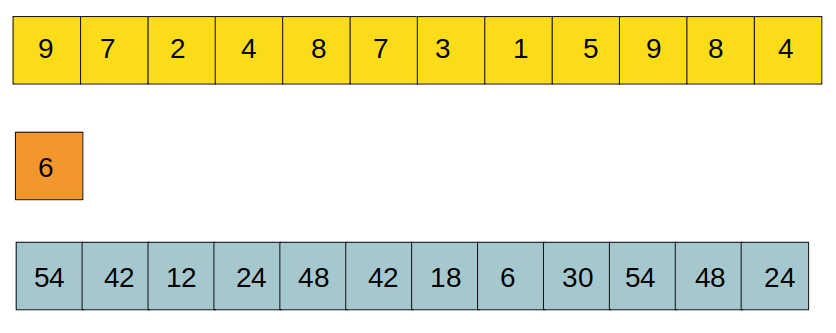
\includegraphics[width=10cm]{figure/conv1d-1.png}
        \caption{Illustration of 1D movement data with depth $1$ and filter size $1$. }
    \end{figure}
\framebreak
    \begin{figure}
        \centering
        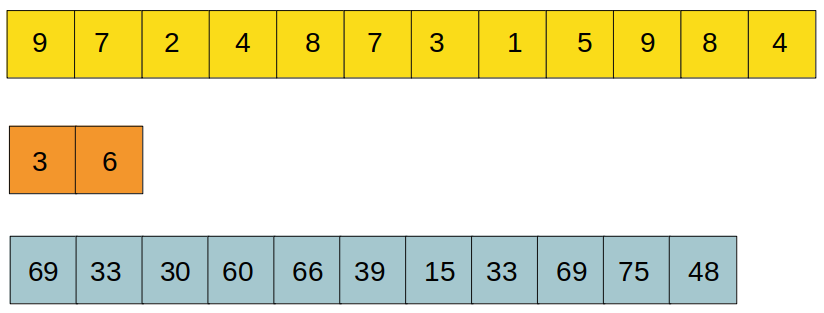
\includegraphics[width=10cm]{figure/conv1d-2.png}
        \caption{Illustration of 1D movement data with depth $1$ and filter size $2$. }
    \end{figure}
\end{vbframe}
%%%%%%%%%%%%%%%%%%%%%%%%%%%%%%%%%%%%%%%%%%%%%%%%%%

\begin{vbframe}{1D Convolutions -- Sensor data}
    \begin{figure}
        \centering
        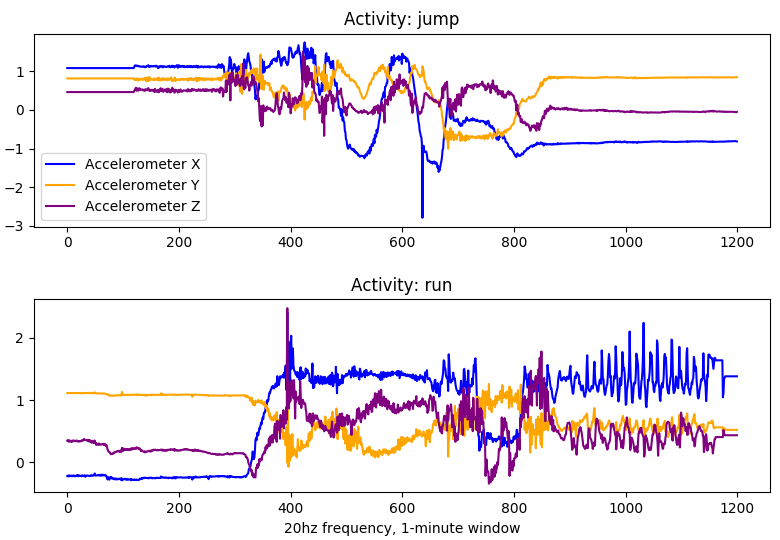
\includegraphics[width=9cm]{plots/05_conv_variations/1d/HAR.png}
        \caption{Illustration of 1D movement data with depth $3$ measured with an accelerometer sensor belonging to a human activity recognition task. }
    \end{figure}
\framebreak
    \begin{figure}
        \centering
        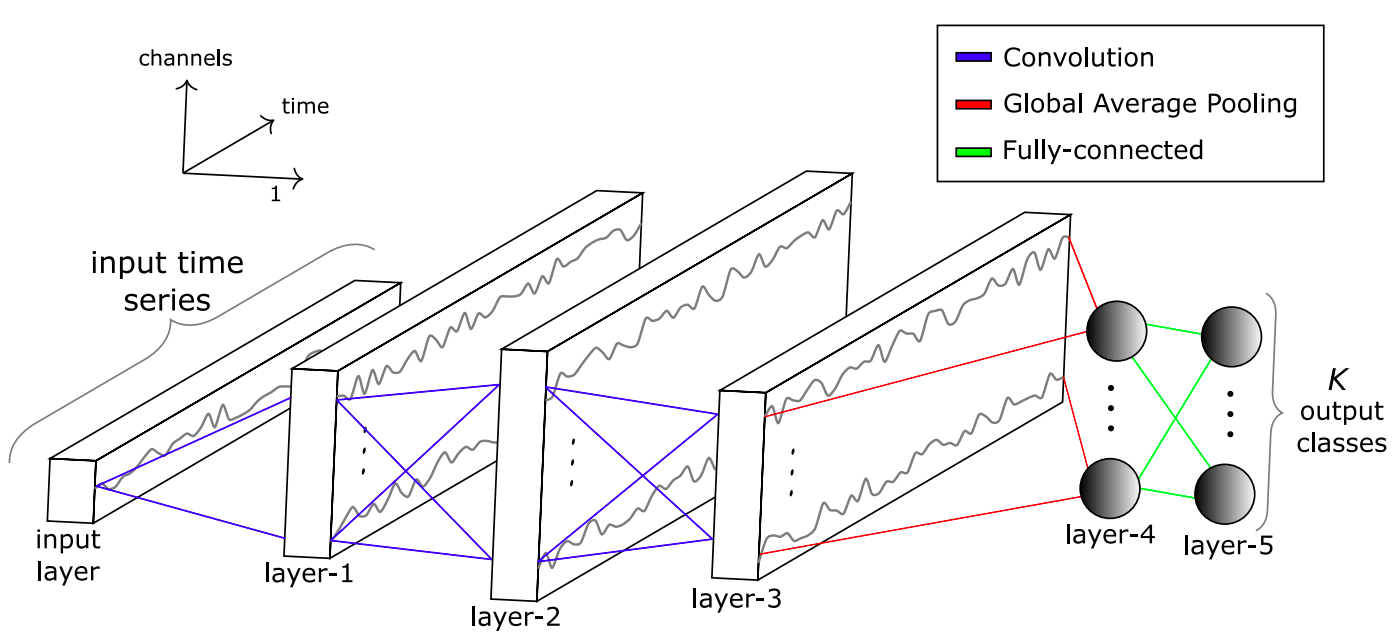
\includegraphics[width=10cm]{plots/05_conv_variations/1d/deep_tsc.png}
        \caption{Time series classification with 1D CNNs and global average pooling (explained later). An input time series is convolved with 3 CNN layers, pooled and fed into a fully connected layer before the final softmax layer. This is one of the classic time series classification architectures (Fawaz et al., 2019).}
    \end{figure}
\end{vbframe}
%%%%%%%%%%%%%%%%%%%%%%%%%%%%%%%%%%%%%%%%%%%%%%%%%%%%%

\begin{vbframe}{1D Convolutions -- Text mining}
    \begin{itemize}
        \item 1D convolutions also have an interesting application in text mining.
        \item For example, they can be used to classify the sentiment of text snippets such as yelp reviews.
    \end{itemize}
    \begin{figure}
        \centering
        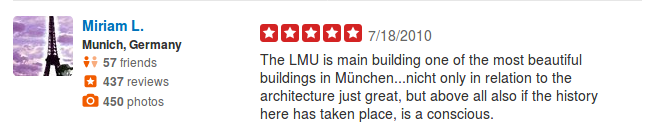
\includegraphics[width=12cm]{plots/05_conv_variations/1d/yelp_lmu.png}
        \caption{Sentiment classification: can we teach the net that this a positive review (Yelp, 2010)?}
    \end{figure}
\end{vbframe}
%%%%%%%%%%%%%%%%%%%%%%%%%%%%%%%%%%%%%%%%%%%%%%%%

\frame{
\frametitle{1D Convolutions -- Text mining}    
    \center
    \only<1>{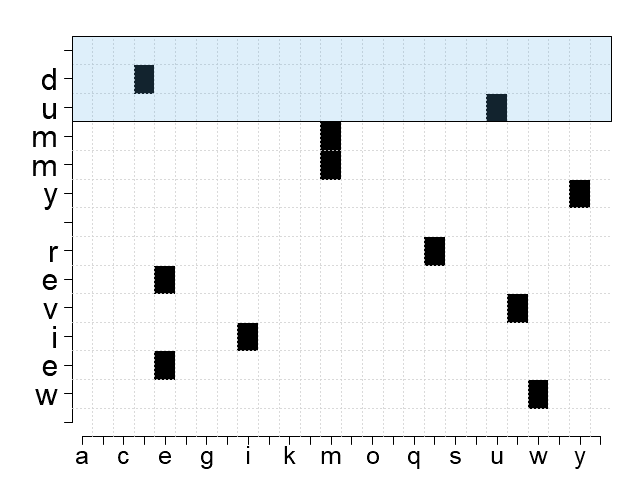
\includegraphics[width=5cm]{plots/text_encoding/1_encoded_text.png}}%
    \only<2>{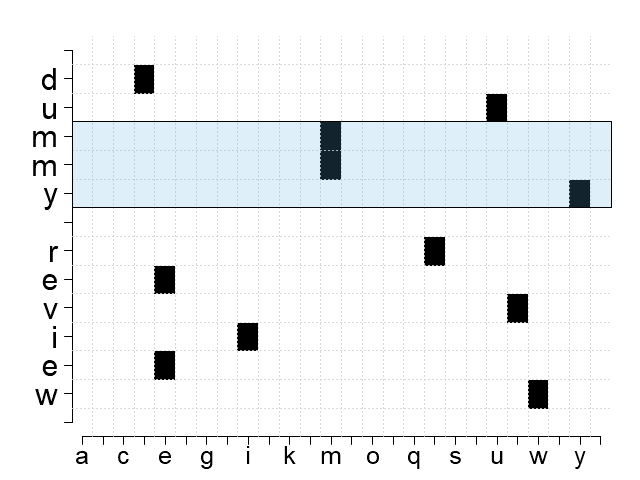
\includegraphics[width=9cm]{plots/text_encoding/4_encoded_text.png}}%
    \only<3>{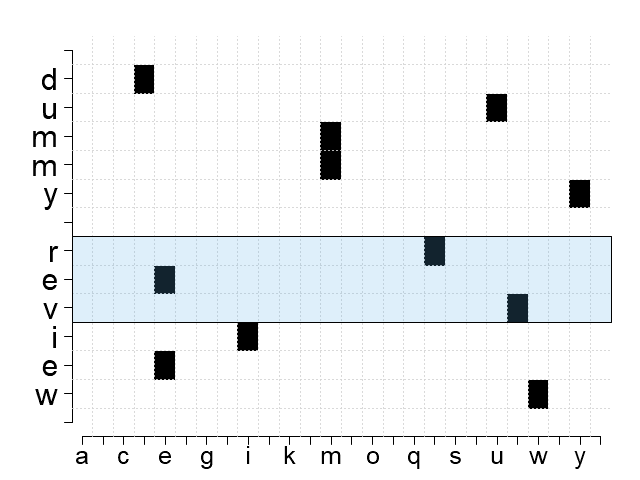
\includegraphics[width=9cm]{plots/text_encoding/8_encoded_text.png}}%
    \only<4>{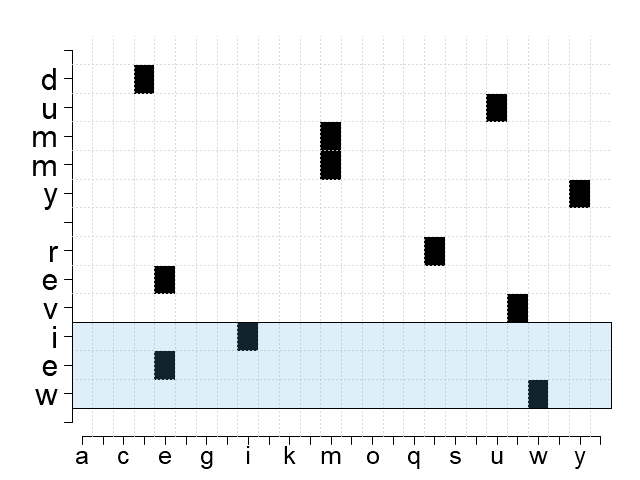
\includegraphics[width=9cm]{plots/text_encoding/11_encoded_text.png}}%
    \\
    % \only<1>{1D convolution of text that was encoded on a character-level. The data is represented as 1D signal with channel size = size of the alphabet as shown in \cite{20}. The temporal dimension is shown as the y dimension for illustrative purposes. The 1D-kernel (blue) convolves the input in the temporal y-dimension yielding a 1D feature vector}  
    \begin{itemize}
        \only<1>{\item We use a given alphabet to encode the text reviews (here: \textit{\enquote{dummy review}}).}
        \only<1>{\item Each character is transformed into a one-hot vector. The vector for character \textit{d} contains only 0's at all positions except for the 4th position.}
        \only<1>{\item The maximum length of each review is set to 1014: shorter texts are padded with spaces (zero-vectors), longer texts are simply cut.}
        \only<2>{\item The data is represented as 1D signal with \emph{depth = size of the alphabet} .}
        \only<3>{\item The temporal dimension is shown as the y dimension for illustrative purposes. }
        \only<4>{\item The 1D-kernel (blue) convolves the input in the temporal y-dimension yielding a 1D feature vector. }
    \end{itemize}
}
%%%%%%%%%%%%%%%%%%%%%%%%%%%%%%%%%%%%%%%%%%%%%%%%

\begin{vbframe}{Advantages of 1D Convolutions}

For certain applications 1D CNNs are advantageous and thus preferable to their 2D counterparts:

   \begin{itemize}
     \item Computational complexity: Forward propagation and backward propagation in 1D CNNs require simple array operations. 
     \item Training is easier: Recent studies show that 1D CNNs with relatively shallow architectures are able to learn challenging tasks involving 1D signals.
     \item Hardware: Usually, training deep 2D CNNs requires special hardware setup (e.g. Cloud computing). However, any CPU implementation over a standard computer is feasible and relatively fast for training compact 1D CNNs.
     \item Application: Due to their low computational requirements, compact 1D CNNs are well-suited for real-time and low-cost applications especially on mobile or hand-held devices.

     \end{itemize}

%The first two advantages can be observed in the previous examples. After 1 $\times$ 1 convolution, we significantly reduce the dimension depth-wise. Say if the original input has 200 channels, the 1  $\times$ 1 convolution will embed these channels (features) into a single channel. 

%The third advantage comes in as after the 1  $\times$ 1 convolution, non-linear activation such as ReLU can be added. The non-linearity allows the network to learn more complex function.

\end{vbframe}

%%%%%%%%%%%%%%%%%%%%%%%%%%%%%%%%%%%%%%%%%%%%%%%
\section{2D Convolutions}
%%%%%%%%%%%%%%%%%%%%%%%%%%%%%%%%%%%%%%%%%%

\begin{vbframe}{2D Convolutions}

The basic idea behind a 2D convolution is sliding a small window (called a "kernel/filter") over a larger 2D array, and performing a dot product between the filter elements and the corresponding input array elements at every position.
    \begin{figure}
        \centering
        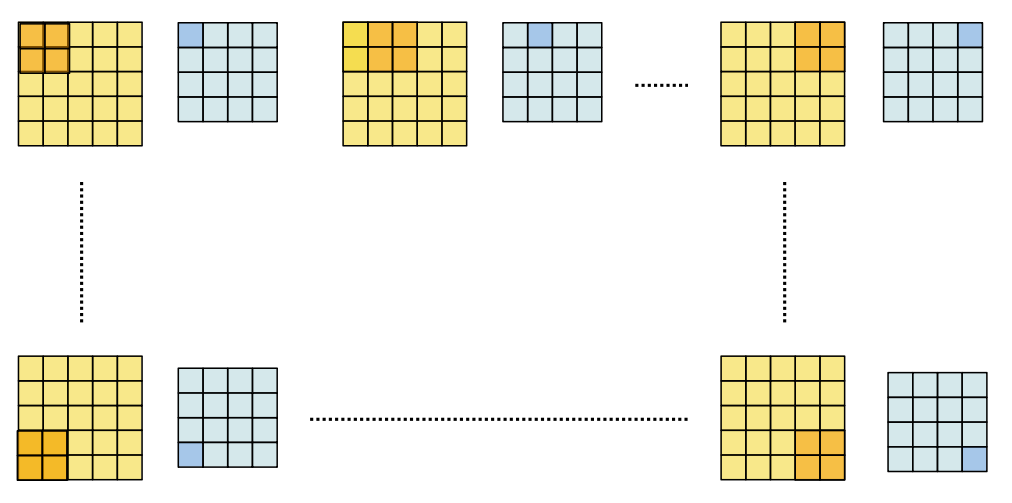
\includegraphics[width=9cm]{figure/padding3.png}
        \caption{\tiny Here's a diagram demonstrating the application of a 2$\times$2 convolution filter to a 5$\times$5 array, in 16 different positions.}
    \end{figure}
\end{vbframe}
%%%%%%%%%%%%%%%%%%%%%%%%%%%%%%%%%%%%%%%%%%%%%%

\frame{
\frametitle{2D Convolutions -- Example}  
    \center
    \only<1>{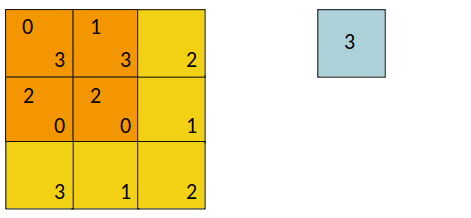
\includegraphics[width=9cm]{figure/conv2d-1.png}}%
    \only<2>{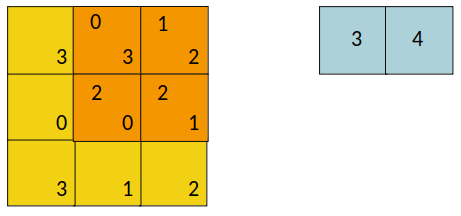
\includegraphics[width=9cm]{figure/conv2d-2.png}}%
    \only<3>{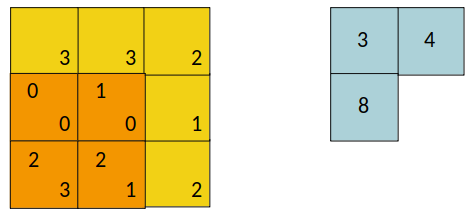
\includegraphics[width=9cm]{figure/conv2d-3.png}}%
    \only<4>{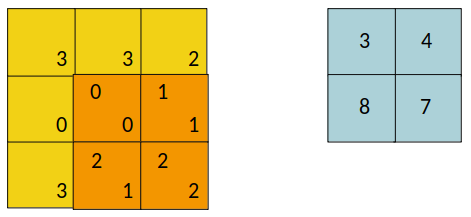
\includegraphics[width=9cm]{figure/conv2d-4.png}}%
    \begin{itemize}
        \only<1>{\item In Deep Learning, convolution is the element-wise multiplication and addition.}
        \only<1>{\item For an image with 1 channel, the convolution is demonstrated in the figure below. Here the filter is a 2$\times$2 matrix with element [[0, 1], [2, 2]].}
        \only<2>{\item The filter is sliding through the input.}
        \only<2>{\item We move/convolve filter on input neurons to create a feature map.}
        \only<3>{\item Notice that stride is 1 and padding is 0 in this example.}
        \only<4>{\item Each sliding position ends up with one number. The final output is then a 2 $\times$ 2 matrix.}
    \end{itemize}
}

%%%%%%%%%%%%%%%%%%%%%%%%%%%%%%%%%%%%%%%%%%%%%%%%%%%%

\section{3D Convolutions}

\begin{vbframe}{3D Convolutions}

\textbf{Data situation}: 3-dimensional tensor data.

    \begin{itemize}
        \item Data consists of tensors with shape [depth, xdim, ydim, zdim].
        \item Dimensions can be both temporal (e.g. video frames) or spatial (e.g. MRI)
        \item Examples:
        \begin{itemize}
            \item Human activity recognition in video data
            \item Disease classification or tumor segmentation on MRI scans
        \end{itemize}
    \end{itemize}

\textbf{Solution}: Move a 3D-kernel in $x$, $y$ and $z$ direction to capture all important information.

\end{vbframe}
%%%%%%%%%%%%%%%%%%%%%%%%%%%%%%%%%%%%%%%%%%%%%%%%
\begin{vbframe}{3D Convolutions -- Data}
    \begin{figure}
        \centering
        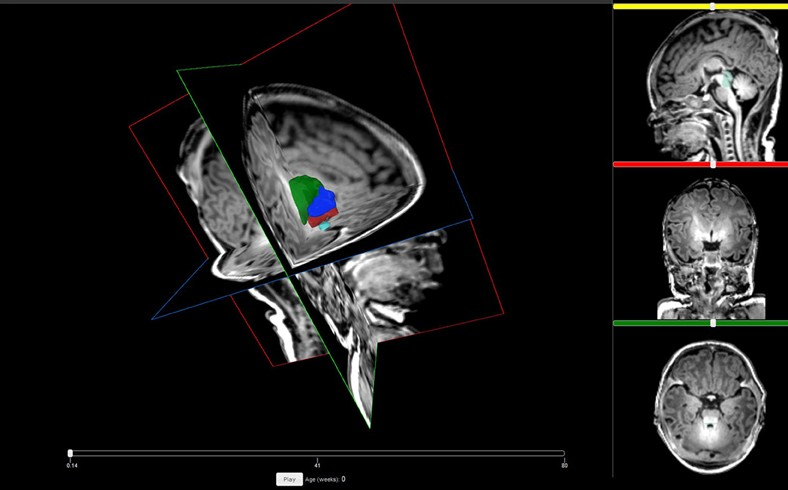
\includegraphics[width=5cm]{plots/05_conv_variations/3d/mri.jpg}
        \caption{Illustration of depth $1$ volumetric data: MRI scan. Each slice of the stack has depth $1$, as the frames are black-white (Gutman et al., 2014).}
    \end{figure}
\end{vbframe}

\begin{vbframe}{3D Convolutions -- Data}
    \begin{figure}
        \centering
        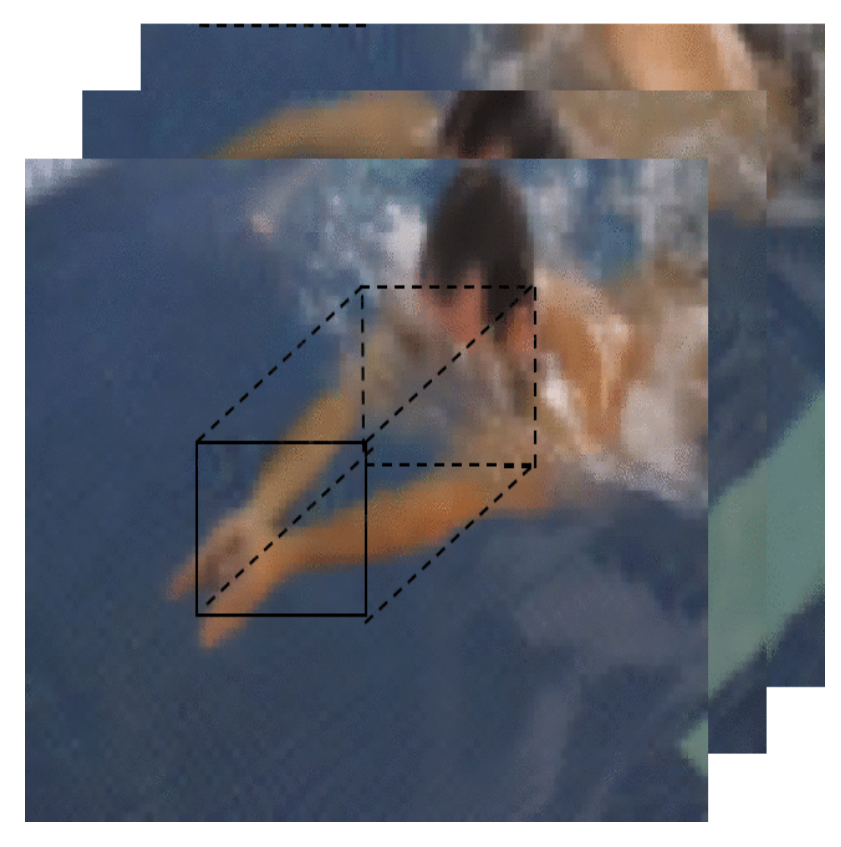
\includegraphics[width=5cm]{plots/05_conv_variations/3d/swim.png}
        \caption{Illustration of volumetric data with depth $> 1$: video snippet of an action detection task. The video consists of several slices, stacked in temporal order. Frames have depth $3$, as they are RGB (Ghosh, 2018).}
    \end{figure}
\end{vbframe}
%%%%%%%%%%%%%%%%%%%%%%%%%%%%%%%%%%%%%%%%%%%%%%%%%

\begin{vbframe}{3D Convolutions}
    \begin{figure}
        \centering
        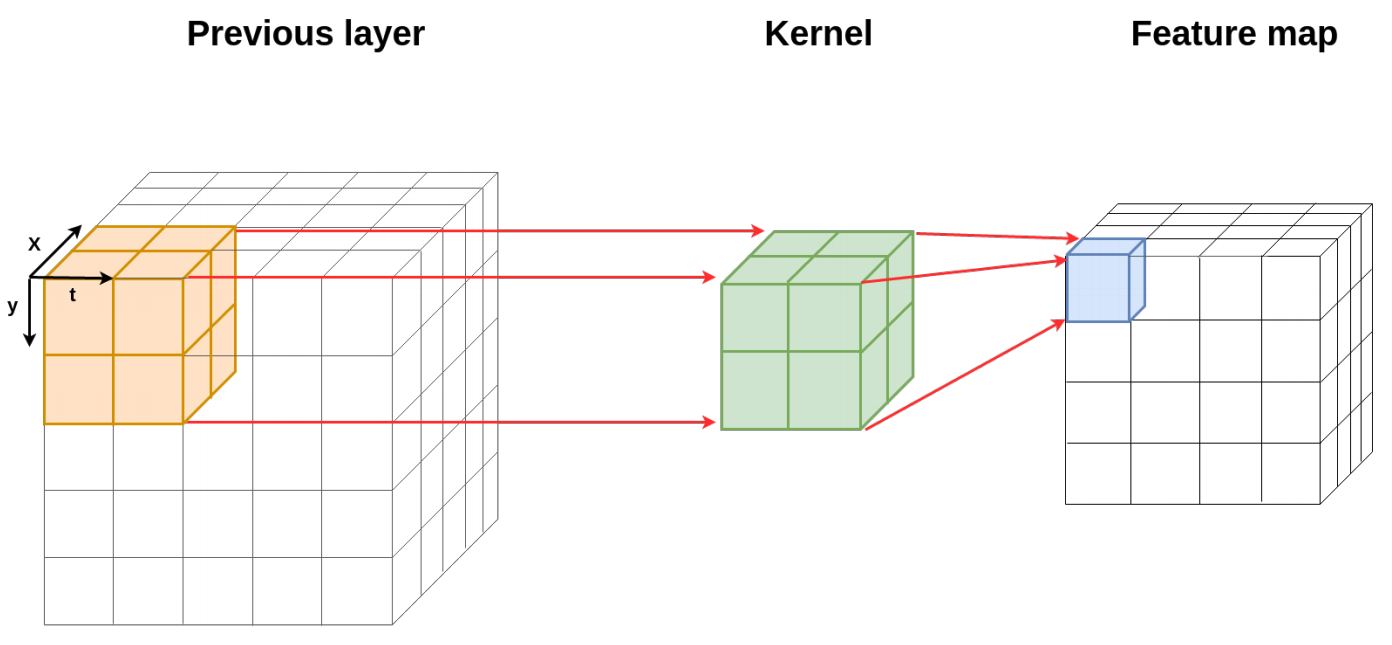
\includegraphics[width=8cm]{plots/05_conv_variations/3d/3dconv.png}
    \end{figure}
    \begin{itemize}
        \item Note: 3D convolutions yield a 3D output (Jin et al., 2023).
        % \item 3D convolution can be expressed as: 
        % $$ H(i, j, k) = (\mathcal{I}\star\mathcal{G})(i, j, k)=\sum_{x}\sum_{y}\sum_{z}\mathcal{I}(x, y, z)\mathcal{G}(i-x, j-y, k-z) $$
    \end{itemize}
\end{vbframe}

\begin{vbframe}{3D Convolutions}
    % https://dspace.cc.tut.fi/dpub/bitstream/handle/123456789/24703/teivas.pdf?sequence=1&isAllowed=y
    \begin{figure}
        \centering
        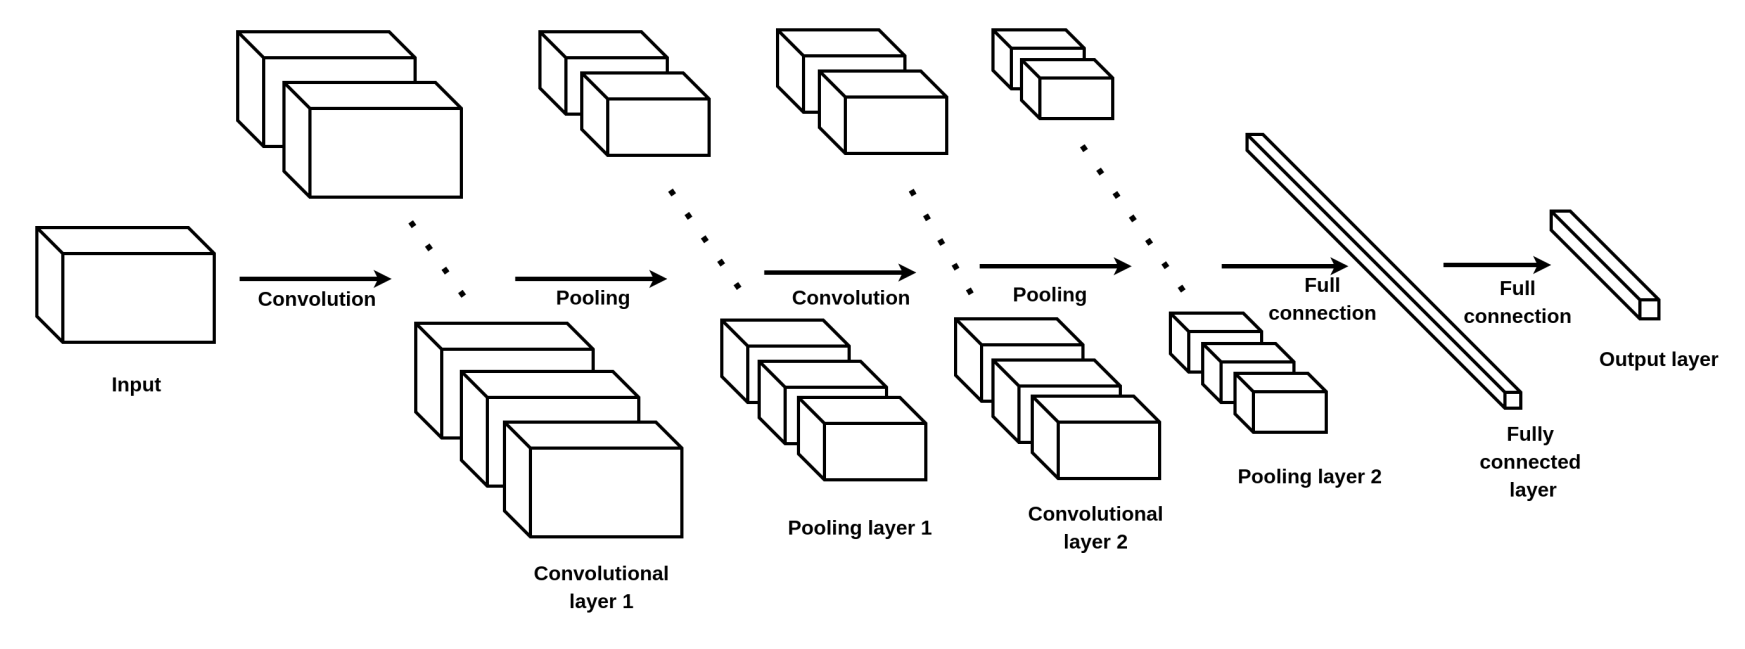
\includegraphics[width=11cm]{plots/05_conv_variations/3d/3dconv_arch.png}
        \caption{Basic 3D-CNN architecture.}
    \end{figure}
    \begin{itemize}
        \item Basic architecture of the CNN stays the same.
        \item 3D convolutions output 3D feature maps which are element-wise activated and then (eventually) pooled in 3 dimensions.
    \end{itemize}
\end{vbframe}
%%%%%%%%%%%%%%%%%%%%%%%%%%%%%%%%%%%%%%%%%%%%%

%%%%%%%%%%%%%%%%%%%%%%%%%%%%%%%%%%%%%%%%%%%%%%%%%%%%%%%%%%%%%%%%%%
%%%%%%%%%%%%%%%%%%%%%%%%%%%%%%%%%%%%%%%%%%%%%%%%%%%%%%%%%%%%%%%%%%
%%%%%%%%%%%%%%%%%%          REFERENCES          %%%%%%%%%%%%%%%%%%
%%%%%%%%%%%%%%%%%%%%%%%%%%%%%%%%%%%%%%%%%%%%%%%%%%%%%%%%%%%%%%%%%%
\begin{vbframe}
\frametitle{References}
\footnotesize{
\begin{thebibliography}{99}
\bibitem[(Ismail Fawaz et al., 2019)]{1}Ismail Fawaz, H., Forestier, G., Weber, J., Idoumghar, L., \& Muller, P.-A. (2019). Deep learning for time series classification: a review. \textit{Data Mining and Knowledge Discovery}, 33. \url{https://doi.org/10.1007/s10618-019-00619-1}

\bibitem[(Gutman et al., 2014)]{2} Gutman, D., Dunn Jr, W., Cobb, J., Stoner, R., Kalpathy-Cramer, J., \& Erickson, B. (2014). Web based tools for visualizing imaging data and development of XNATView, a zero footprint image viewer. \textit{Frontiers in Neuroinformatics}, 8, 53. \url{https://doi.org/10.3389/fninf.2014.00053}

\bibitem[(Ghosh, 2018)] {3}Ghosh, R. (2018, June 11). Deep learning for videos: A 2018 guide to action recognition. Deep Learning for Videos: A 2018 Guide to Action Recognition. https://blog.qure.ai/notes/deep-learning-for-videos-action-recognition-review 


\bibitem[(Jin et al., 2023)]{4} Jin, X., Yang, H., He, X., Liu, G., Yan, Z., \& Wang, Q. (2023). Robust LiDAR-Based Vehicle Detection for On-Road Autonomous Driving. \textit{Remote Sensing, 15}(12). \url{https://doi.org/10.3390/rs15123160}

\bibitem[(Yelp, 2010)]{2}Yelp. (2010). \textit{Ludwig-Maximilians-Universität München - Munich}. \url{https://www.yelp.com/biz/ludwig-maximilians-universit%C3%A4t-m%C3%BCnchen-m%C3%BCnchen-2} 

% \bibitem[Dumoulin et al., 2016]{14} Dumoulin, Vincent and Visin, Francesco (2016)
% \newblock A guide to convolution arithmetic for deep learning
% \newblock \emph{\url{https://arxiv.org/abs/1603.07285v1}}
% %%%%%%%%%%%%%%%%%%%%%%%%%%%%%%%%%%
% \bibitem[van den Oord et al., 2016]{15} Van den Oord, Aaron, Sander Dielman, Karen Simonyan, Oriol Vinyals, Alex Graves, Nal Kalchbrenner, and Koray Kavukocuoglu (2016)
% \newblock WaveNet: A Generative Model for Raw Audio
% \newblock \emph{\url{https://arxiv.org/abs/1609.03499}}
% %%%%%%%%%%%%%%%%%%%%%%%%%%%%%%%%%%
% %%%%%%%%%%%%%%%%%%%%%%%%%%%%%%%%%%
% \bibitem[Gennart et al., 1996]{17} Benoit A., Gennart, Bernard Krummenacher, Roger D. Hersch, Bernard Saugy, J.C. Hadorn and D. Mueller (1996)
% \newblock The Giga View Multiprocessor Multidisk Image Server
% \newblock \emph{\url{https://www.researchgate.net/publication/220060811_The_Giga_View_Multiprocessor_Multidisk_Image_Server}}
% %%%%%%%%%%%%%%%%%%%%%%%%%%%%%%%%%%
% %%%%%%%%%%%%%%%%%%%%%%%%%%%%%%%%%%
% \bibitem[Tran et al., 2015]{18} Tran, Du, Lubomir Bourdev, Rob Fergus,  Lorenzo Torresani and Paluri Manohar (2015)
% \newblock Learning Spatiotemporal Features with 3D Convolutional Networks
% \newblock \emph{\url{https://arxiv.org/pdf/1412.0767.pdf}}
% %%%%%%%%%%%%%%%%%%%%%%%%%%%%%%%%%%
% %%%%%%%%%%%%%%%%%%%%%%%%%%%%%%%%%%
% \bibitem[Milletari et al., 2016]{19} Milletari, Fausto, Nassir Navab and  Seyed-Ahmad Ahmadi (2016)
% \newblock V-Net: Fully Convolutional Neural Networks for
% Volumetric Medical Image Segmentation
% \newblock \emph{\url{https://arxiv.org/pdf/1606.04797.pdf}}
% %%%%%%%%%%%%%%%%%%%%%%%%%%%%%%%%%%
% %%%%%%%%%%%%%%%%%%%%%%%%%%%%%%%%%%
% \bibitem[Zhang et al., 2015]{20} Zhang, Xiang, Junbo Zhao and Yann LeCun (2015)
% \newblock Character-level Convolutional Networks for Text Classification
% \newblock \emph{\url{http://arxiv.org/abs/1509.01626}}
% %%%%%%%%%%%%%%%%%%%%%%%%%%%%%%%%%%
% %%%%%%%%%%%%%%%%%%%%%%%%%%%%%%%%%%
% \bibitem[Wang et al., 2017]{21} Wang, Zhiguang, Weizhong Yan and Tim Oates (2017)
% \newblock Time Series Classification from Scratch with Deep Neural Networks: A Strong Baseline
% \newblock \emph{\url{http://arxiv.org/abs/1509.01626}}
% %%%%%%%%%%%%%%%%%%%%%%%%%%%%%%%%%%
% %%%%%%%%%%%%%%%%%%%%%%%%%%%%%%%%%%
% \bibitem[Yu et. al, 2015]{22} Fisher Yu and Vladlen Koltun (2015)
% \newblock Multi-Scale Context Aggregation by Dilated Convolutions
% \newblock \emph{\url{https://arxiv.org/abs/1511.07122}}
% %%%%%%%%%%%%%%%%%%%%%%%%%%%%%%%%%%
% %%%%%%%%%%%%%%%%%%%%%%%%%%%%%%%%%%
% \bibitem[Bai et. al, 2018]{23} Bai, Shaojie,  Zico J. Kolter and Vladlen Koltun (2018)
% \newblock An Empirical Evaluation of Generic Convolutional and Recurrent Networks for Sequence Modeling
% \newblock \emph{\url{http://arxiv.org/abs/1509.01626}}
% %%%%%%%%%%%%%%%%%%%%%%%%%%%%%%%%%%
% %%%%%%%%%%%%%%%%%%%%%%%%%%%%%%%%%%
% \bibitem[Odena et. al , 2017]{24} Augustus Odena, Vincent Dumoulin and Chris Olah (2016)
% \newblock Deconvolution and Checkerboard Artifacts
% \newblock \emph{\url{https://distill.pub/2016/deconv-checkerboard/}{https://distill.pub/2016/deconv-checkerboard/}}
% %%%%%%%%%%%%%%%%%%%%%%%%%%%%%%%%%%
% %%%%%%%%%%%%%%%%%%%%%%%%%%%%%%%%%%
% \bibitem[Arauho et. al , 2019]{45} Andre Araujo, Wade Norris and Jack Sim (2019)
% \newblock Computing Receptive Fields of Convolutional Neural Networks
% \newblock \emph{\url{https://distill.pub/2019/computing-receptive-fields/}}
% %%%%%%%%%%%%%%%%%%%%%%%%%%%%%%%%%%
% %%%%%%%%%%%%%%%%%%%%%%%%%%%%%%%%%%
% \bibitem[Wang et. al , 2017]{31} Zhiguang Wang, Yan, Weizhong and Tim Oates (2017)
% \newblock Time series classification from scratch with deep neural networks: A
% strong baseline
% \newblock \emph{\url{https://arxiv.org/1611.06455}}
% %%%%%%%%%%%%%%%%%%%%%%%%%%%%%%%%%%
% %%%%%%%%%%%%%%%%%%%%%%%%%%%%%%%%%%
% \bibitem[Lin et al., 2017]{38} Lin, Haoning and Shi, Zhenwei and Zou, Zhengxia (2017)
% \newblock Maritime Semantic Labeling of Optical Remote Sensing Images with Multi-Scale Fully Convolutional Network

\end{thebibliography}
}
\end{vbframe}




\endlecture
\end{document}